\documentclass{article}
\usepackage[utf8]{inputenc}
\usepackage[T1]{fontenc}
\usepackage[french]{babel}
\usepackage{amsmath}
\usepackage{amsfonts}
\usepackage{amssymb}
\usepackage{ulem}
\usepackage{float}
\usepackage{graphicx}
\usepackage{subfiles}
\usepackage{subfigure}
\usepackage{color}
\usepackage{soul}
\usepackage[hidelinks]{hyperref}
\usepackage{caption}
\usepackage{tcolorbox}
\usepackage[margin=1in]{geometry} 
\usepackage{booktabs}
\usepackage{geometry}
\usepackage{hyperref}
\usepackage{tablefootnote}
% ajouter tous les package ici
\numberwithin{equation}{section}
\tcbuselibrary{theorems}
\graphicspath{{pics/}}

\title{\begin{figure}[H]
\subfigure{
\label{Logo_isep}

\includegraphics[width = 0.6\textwidth]{Semaine3/Problems2/rapport/pics/logo_isep.png}
}
\subfigure{
\label{Logo_data_waves}

\includegraphics[width = 0.3\textwidth]{Semaine3/Problems2/rapport/pics/logo_data_waves.png}

}
\end{figure}
Traitement numérique du signal \\ \vspace{5mm} Livrable final \\ \vspace{3mm} Groupe G10C } 

\author{MANGIN Rémi \\
LE MONNIER Romain \\
TEOFILOVIC Kristina \\
TON Sophie \\
RISY Théo \\
YANG Chen}   
\date{\today}  
\begin{document}

\maketitle

\newpage
\tableofcontents
\newpage

\textbf{Problème II :} \  \\
Proposer un algorithme qui permet de détecter, de caractériser une note de musique jouée par un instrument (violon, flûte, piano) et de déterminer sa hauteur. \\
Cet algorithme devra produire les sorties suivantes : \\
\begin{itemize}
    \item $t_d, t_f$: instants de début et de fin de note
    \item $P_dBm$: la puissance moyenne du signal en dBm
    \item $f_0$: la fréquence fondamentale et le nom et l'octave de la note jouée
    \item $f_h$: la fréquence haute telle que [0,$f_h$] contient 99.99\% de la puissance
    \item $n_h$: le nombre d'harmoniques dans cette bande de fréquences
    \item Toutes autres caractéristiques qui vous paraît pertinente pour classifier les notes par instrument de musique.
    On reprendra la méthode de détection d'un son utile du PBI et on justifiera les paramètres retenus.
\end{itemize}

\textbf{Problème IV :} \ \\
On souhaite détecter les signaux environnementaux qui comprennent des composantes spectrales très aiguës et pénibles pour l'oreille humaine. Ces signaux sont définis ainsi : 20\% de leur puissance est comprise dans les fréquences supérieures à 2 kHz, avec une puissance sonore totale supérieure à 110 dB SLP. \\
Concevoir un système de détection de ces signaux pénibles fondé sur filtrage
numérique. On prendra un micro de sensibilité égale à -67 dBV et de gain égal à 16 dB. Discuter les critères énoncés.

  
\newpage
\textcolor{blue}{\section{Chapitre I : Problème I}}
\textcolor{blue}{\subsection{Introduction}}
Nous présentons une approche de détection de signaux audio , dont les caractéristiques sont les suivantes :
\begin{itemize}
    \item Un micro avec une sensibilité (S) de - 48 dBV et un Gain (G) de 40 dB.
    \item Les sons pénibles sont définis comme des sons de plus d'une seconde, dépassant une puissance en dBm de référence.
    \item Les sons acceptables sont définis en dessous de ce seuil.
    \item Chaque signal sera caractérisé par sa durée, sa puissance moyenne, tension RMS, et classifié en conséquence. 
\end{itemize}

Les expérimentations seront réalisées sur les signaux de la question F, signaux qui nous ont été fournis (bruit de marteau piqueurs, bruit de ville et de jardin). Dans un premier temps, nous implémenterons le code de détection sur le micro-contrôleur, en choisissant une fréquence d'échantillonnage adaptée aux caractéristiques matérielles. La caractérisation des bruits détectés fera l'objet d'une étape ultérieure.
\newline 
\\
 \textbf{Problème I - Énoncé } \ \\
Proposer un algorithme qui permet de détecter la présence/absence d’un signal audio enregistrant le bruit ambiant.
Le micro utilisé a une sensibilité S (dBV) et amplifie le signal électrique avec un gain G. On définit un son "son pénible", comme un signal sonore de durée supérieure à Dt (s) et de niveau supérieur ou égal à $P_{SPL}$ (dB SPL1). A contrario, un "son acceptable", correspond à un signal sonore de niveau inférieur à $P_{SPL}$.
\\
Caractériser chaque son détecté par :
\begin{itemize}
    \item Sa durée 
    \item sa puissance
    \item sa tension RMS en V et le classifier en "son pénible" ou "son acceptable"
\end{itemize}
Paramètres S = -48 dBV, G = 40 dB, $P_{SPL}$ = 80 dB SPL, $D_t$ = 1s.
\\
Les expérimentations seront menées sur les signaux de la question F.








\newpage
\textcolor{blue}{\subsection{Méthode}}Tout d'abord, il faut définir $P_{dBm}$. Le schéma du microphone qui nous est donné permet de réaliser les calculs.

\begin{figure}[htb]
    \centering
    \includegraphics[width=0.8\textwidth]{schemabloc_méthode1.png}
    \caption{Schéma bloc microphone}
    \label{fig:Schéma_Fonctionnel_1}
\end{figure}

En effet, nous avons la relation suivante :
\begin{equation}
P_{dBm} = 10 \times \log(V_a^2 \times 1000) \ \text{avec}\ V_a = S \times P_a
\end{equation}
Cependant, S la sensibilité \footnote{\href{http://electroacoustique.univ-lemans.fr/cours/Grain1.2/co/grain2_2_2.html}{Pour la formule de la sensibilité S}} que l'on nous donne est en dBV et pas en $V/P_a$, il faut donc la convertir. Nous savons que :\begin{equation}
    S = 20\times \log(\frac{S_{v/Pa}}{S_{ref}}) \ \text{avec}\  S_{ref} = 1 V/P_a
\end{equation} donc :
\begin{equation}
   S_{V/P_a} = S_{ref}*10^\frac{S}{20} 
\end{equation}
Nous avons donc :
\begin{equation}
V_m = S_{V/P_a} \times P_a
\end{equation} 
Pour $P_a$, nous utilisons la formule de $P_{SPL}$ \footnote{\href{https://fr.wikipedia.org/wiki/Pression_acoustique}{Pour la formule de $P_{SPL}$}}: 
\begin{equation}
    P_{SPL} = 20\times \log(\frac{P_a}{P_{ref}}) 
\end{equation}
d'où :
\begin{equation}
P_a = P_{ref} * 10^{\frac{P_{SPL}}{20}}
\end{equation}
Il ne reste que le gain à traiter, celui-ci s'exprime en dB dans les paramètres donnés, or, nous voulons l'exprimer sans unité, nous obtenons alors 
\begin{equation}
    G_{SU} = 10^\frac{G}{20} \ \text{où} \ G_{SU} \ \text{est sans unité} \footnote{\href{https://fr.wikipedia.org/wiki/Gain_d\%C3\%A9cibel}{Pour la formule du gain sans unité $G_{SU}$}}
\end{equation}

Cela nous permet de trouver la formule finale : 
\\
\tcbox[colback=yellow!20, colframe=yellow, boxrule=2pt]{$ P_{dBm} = 10 \times \log((G_{SU} \times S_{VPA} \times P_a)^2 \times 1000)$}

En substituant avec les résultats précédents, on obtient :
\tcbox[colback=green!20, colframe=green, boxrule=2pt]{$P_{dBm} = 20 \times \log(10^\frac{G}{20} \times S_{REF} \times 10^{\frac{S}{20}} \times P_{REF} \times 10^{\frac{P_{SPL}}{20}})+30$}
Enfin, avec : \begin{itemize}
    \item $S_{REF} = 1$
    \item $P_{REF} = 20 \mu Pa$
    \item $G = 40 dB$
    \item $S = -48 dBV$
    \item $P_{SPL} = 80 dB SPL$
\end{itemize} 
On obtient : \tcbox[colback=green!20, colframe=green, boxrule=2pt]{$P_{dBm} = 8 dBm$.}
À présent, nous avons la valeur de $P_{dBm}$ qui va nous servir de référence. Pour chaque signal, nous allons le décomposer en plusieurs « sous-signaux » à chaque fois que la valeur de référence est franchie. 
Par exemple, sur la figure \ref{Fig.1.2}, on distingue trois « sous-signaux » ou plages de signal différentes, car la valeur de référence est franchie deux fois. Ensuite, chaque plage est traitée comme un nouveau signal et, si cette plage se trouve au-dessus de la valeur référence et dure plus d’une seconde, alors le son de cette plage est catalogué dans la catégorie bruit pénible. Sur cet exemple, il y a donc deux sons acceptables (plages 1,3) et un son pénible (plage 2).
Enfin, pour chaque signal, on règle la taille des fenêtres d’analyse pour obtenir un résultat correct, contenant 2k+1 échantillons.Pour déterminer la puissance instantanée, nous utilisons la formule suivante :
\begin{equation}
    P(n) = \frac{1}{2K+1}\sum_{n-K}^{n+K}_{x(k)^2}
\end{equation}
L'identification du paramètre k ainsi que le choix de sa valeur retenue dépendent de la nature du signal et des exigences spécifiques de l'analyse. Admettons que nous avons un signal de 5s et d'une fréquence de 20k Hz, si k = 80, on aura 161 échantillons par fenêtre. Pour un signal sonore, il faut que la taille de la fenêtre soit petite, car c'est un fichier son. Pour avoir un bon vecteur puissance à analyser, il faut donc une fenêtre inférieure à la seconde, comme on a Te, il faut déterminer k tel que :
\begin{equation}
    k < \frac{(\frac{1}{Te}-1)}{2}
\end{equation}
\begin{figure}[htb]
    \centering
    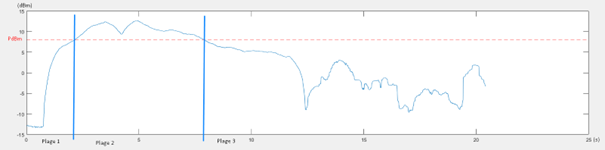
\includegraphics[width=0.8\textwidth]{Exemple_seuil_se_pénibilité.png}
    \caption{Exemple signal avec plages acceptables et pénibles}
    \label{Fig.1.2}
\end{figure}


\newpage
\textcolor{blue}{\subsection{Résultats Expérimentaux}}
Après avoir appliqué la fonction du problème aux signaux Jardin01.mp3, Jardin02.mp3, Ville01.mp3 et MarteauPiqueur01.mp3, voici ce que nous obtenons :
\\
\\
\textbf{Légende :}
\\
\textcolor{red}{Rouge :} dépasse la durée et la puissance seuil
\\
\textcolor{blue}{Bleu : }dépasse la puissance seuil, mais plus petit que dt

\begin{figure}[htb]
\subfigure[Application sur le signal Jardin01]{
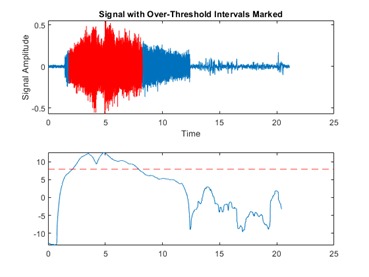
\includegraphics[width = 0.45\textwidth]{jardin01.png}
\label{Fig.sub.1.3.1}
}
\subfigure[Application sur le signal Jardin02]{
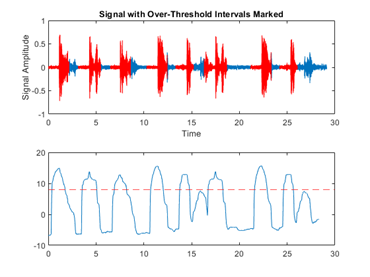
\includegraphics[width = 0.45\textwidth]{jardin02.png}
\label{Fig.sub.1.3.2}
}
\subfigure[Application sur le signal MarteauPiqueur]{
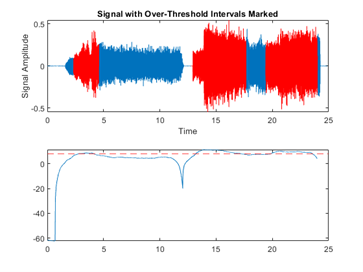
\includegraphics[width = 0.45\textwidth]{marteaaupiqueur01.png}
\label{Fig.sub.1.3.3}
}
\subfigure[Application sur le signal Ville01]{
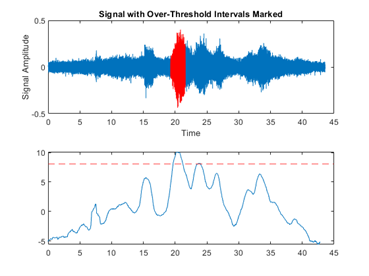
\includegraphics[width = 0.45\textwidth]{ville01.png}
\label{Fig.sub.1.3.4}
}
\caption{Application sur les signaux donnés}
\label{Fig.main.2}
\end{figure}

Pour chacun des signaux, l'amplitude en fonction du temps est présentée en haut, tandis que la puissance en dBm en fonction du temps est affichée en bas. Les pointillés rouges désignent la puissance de référence à 8 dBm et nous observons bien que lorsque le signal dépasse 8 dBm et dure plus d'une seconde, nous avons une plage de son pénible (en rouge).
\\
\\
\begin{table}
  \centering
  \begin{tabular}{|c|c|c|c|c|}
    \hline
    & Ville01 & MarteauPiqueur01 & Jardin01 & Jardin02 \\
    \hline
    Puissance moyenne (dBm) &-27.363 & -22.7752 
  &-23.5662 & -21.5499\\
    \hline
    Puissance moyenne (mW) & 1.835 & 5.2781\times 10^-6 & 4.3992\times10^-6 & 6.9986\times10^-6\\
    \hline
    Durée & 43.5566 & 24.8176 & 21.058 & 29.0993\\
    \hline
    Tension RMS (V) & 0.0013547 & 0.0022974 & 0.0020974 & 0.0026455 \\
    \hline
  \end{tabular}
    \caption{Avant Amplification}
\end{table}
\\
\begin{table}
  \centering
  \begin{tabular}{|c|c|c|c|c|}
    \hline
    & Ville01 & MarteauPiqueur01 & Jardin01 & Jardin02 \\
    \hline
    Puissance moyenne (dBm) & 12.637 & 17.2248 & 16.4338 & 18.4501\\
    \hline
    Puissance moyenne (mW) & 0.018353 & 0.052781 & 0.043992& 0.069986\\
    \hline
    Durée (s)& 43.5566 & 24.8176 & 21.058 & 29.0993 \\
    \hline
    Tension RMS (V) & 0.13547 & 0.22974 & 0.20974 & 0.26455 \\
    \hline
  \end{tabular}
    \caption{Après Amplification}
\end{table}
\\
\newpage
% analyse des sons par rapport au ressenti à l'oreille sons pénible par rapport aux programme 
Dans ce tableau des caractéristiques des différents signaux, nous avons déterminé la puissance moyenne. Elle mesure la puissance d'un signal sur une période de temps donnée et elle est définie comme la quantité totale d'énergie transférée ou consommée divisée par la durée de cette période. Entre deux instants, elle est l'énergie dissipée par la durée d'observation et sa formule est : 
\begin{equation}
    P(x, t_{1}, t_{2}) = \frac{1}{t_{2} - t{1}} \int_{t_{1}}^{t_{2}}x_{c}(t)^2 dt
\end{equation}
\newpage
\textcolor{blue}{\subsection{Conclusion}}
Pour conclure, le problème 1 a été abordé à travers la conception d’un algorithme dédié à la détection de la présence ou de l’absence de signaux audio, enregistrant ainsi le bruit ambiant. Nos expérimentations ont débuté en utilisant des sons préalablement définis, fournis dans la question F, tels que des bruits de marteau-piqueur, de ville, et de jardin 1 et 2. L’analyse approfondie de ces sons a permis de classer les signaux en deux catégories distinctes : les "sons pénibles", identifiés en rouge, définis par une durée excédant à 1 seconde et une puissance en dBm égale ou supérieure à 8, et les "sons acceptables" distingués en bleu, caractérisés par une puissance en dBm inférieure à ce seuil. 
\\

Nos résultats présentent des points forts notables. La méthode de classification des signaux a démontré une clarté visuelle, facilitée par l'utilisation de couleurs, renforçant ainsi la compréhension des différentes catégories. De plus, la caractérisation détaillée de chaque signal fournit une base solide pour évaluer l'impact des sons sur l'environnement.
\\

Cependant, des points faibles nécessitent une attention particulière. La détermination du seuil de puissance pour les "sons pénibles" pourrait être améliorée pour refléter davantage la variabilité des environnements sonores. De plus, la limitation actuelle de nos expérimentations à des enregistrements préétablis soulève des questions sur la généralisation de notre algorithme à des situations en temps réel et dynamique.
\\

Pour perfectionner notre recherche, nous envisageons d'optimiser la calibration du seuil de puissance en tenant compte de la variabilité environnementale. L'extension de nos expérimentations à des conditions réelles d'environnement sonore permettra une validation plus approfondie de notre algorithme. Ces perspectives d'amélioration visent à renforcer la fiabilité et l'applicabilité de notre méthode dans des situations plus diversifiées et changeantes.

\newpage
\textcolor{blue}{\section{Chapitre II : Problème II}}
\textcolor{blue}{\subsection{Introduction}}
Nous proposons une approche novatrice visant à élaborer un algorithme de détection et de caractérisation des notes de musique jouées par divers instruments tels que le violon, la flûte et le piano, tout en déterminant précisément leur hauteur. Notre algorithme est conçu pour générer des sorties exhaustives, incluant les instants de début et de fin de chaque note ($t_d$,$t_f$), la puissance moyenne du signal en dBm ($P_{dBm}$), la fréquence fondamentale ($f_0$) accompagnée du nom et de l’octave de la note jouée, la fréquence haute $f_h$ définie par [0, $f_h$] englobant 99.99\% de la puissance, le nombre d’harmoniques dans cette bande de fréquences ($n_h$), ainsi que toute autre caractéristique jugée pertinente pour classifier les notes selon l'instrument de musique. Nous adopterons la méthode de détection d’un son utile du PBI (Produit de l'analyse du Bruit Instantané) pour élaborer notre algorithme, en nous appuyant sur une approche en trois étapes. Cette méthodologie implique la détection du signal sonore, la synchronisation du récepteur par la détection de l'en-tête, et enfin, le décodage des informations pertinentes pour caractériser chaque note. 

\newpage
\textcolor{blue}{\subsection{Méthode}}

Les signaux originales sont en stéréo, il faut les moyenner pour retrouver dans le cadre du cours.
fig.\ref{Fig.sub.1} est le signal avant moyenner, fig.\ref{Fig.sub.2} est le singal après moyenner.
\begin{figure}[htb]
\subfigure[Exemple de signal audio original]{
\label{Fig.sub.1}
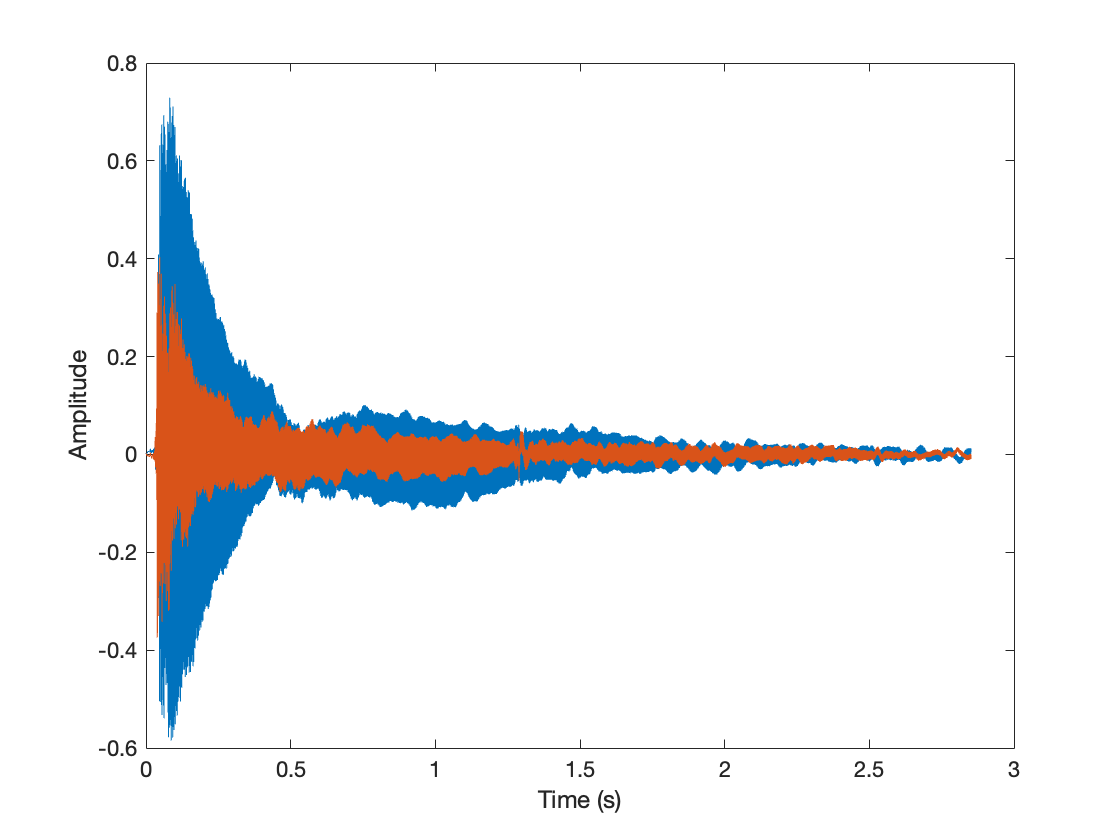
\includegraphics[width = 0.45\textwidth]{signal_before_mean.png}
}
\subfigure[Exemple de signal après moyenner]{
\label{Fig.sub.2}
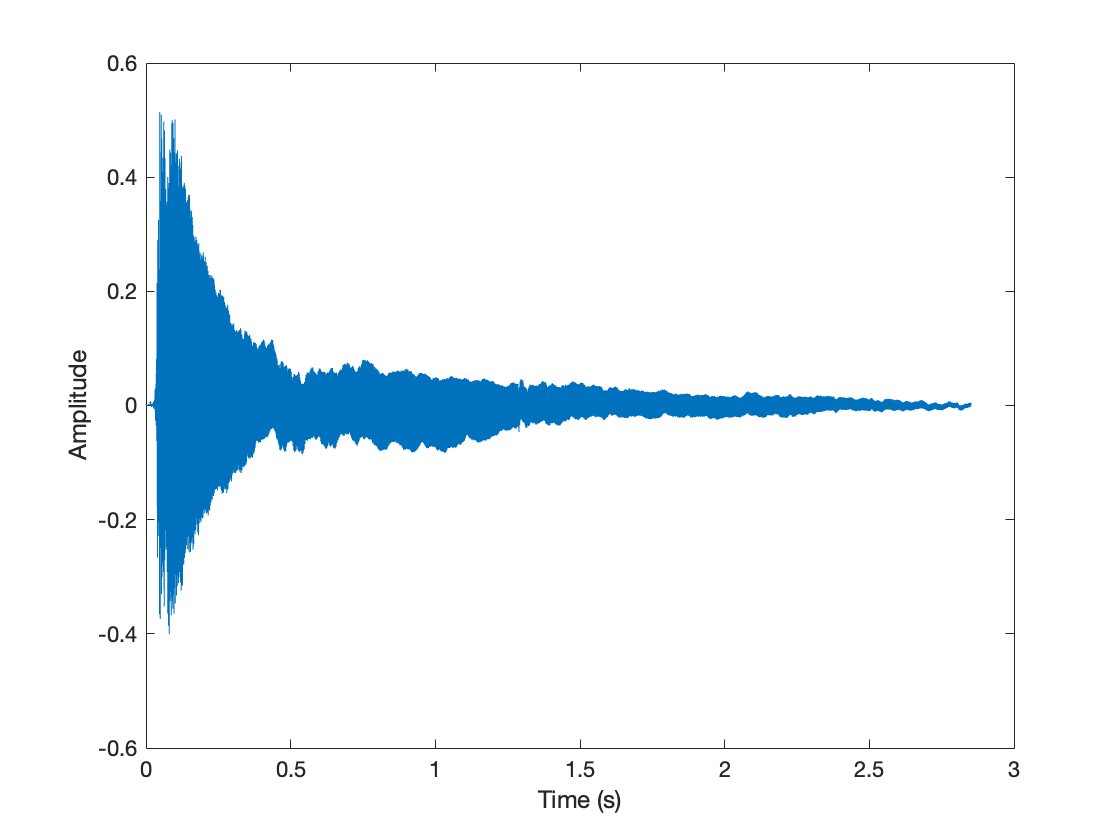
\includegraphics[width = 0.45\textwidth]{signal_after_mean.png}
}
\caption{Exemple de signal}
\label{Fig.main}
    % ici c'est le problem de overleaf que l'image ne marche pas
\end{figure}

\textcolor{blue}{\subsubsection{Acquisition et Pré-traitement du Signal}}

Dans cette première étape, nous chargeons une série de fichiers audio correspondant à différentes notes jouées par des instruments tels que le violon, la flûte et le piano. Ces fichiers audio sont ensuite convertis en signaux mono pour simplifier l'analyse. Pour chaque signal, nous calculons la puissance du signal en utilisant une fenêtre glissante de taille fixe. La puissance ainsi obtenue est ensuite convertie en décibels (dB). Ce processus est essentiel pour préparer le signal en vue de l'analyse ultérieure. 
\newpage
\textcolor{blue}{\subsubsection{Détection des Notes}}
La détection se fait en trouvant les points où la puissance du signal dépasse un seuil défini (1\% de la puissance maximale). Les indices correspondants sont ensuite convertis en temps, fournissant ainsi les instants de début et de fin de chaque note. Les notes d'une durée inférieure à une seconde sont éliminées pour garantir la qualité des données. 
Fig.\ref{fig:Note_Detection} est le signal avec les notes détectées(partie rouge).
\begin{figure}[htb]
    \centering
    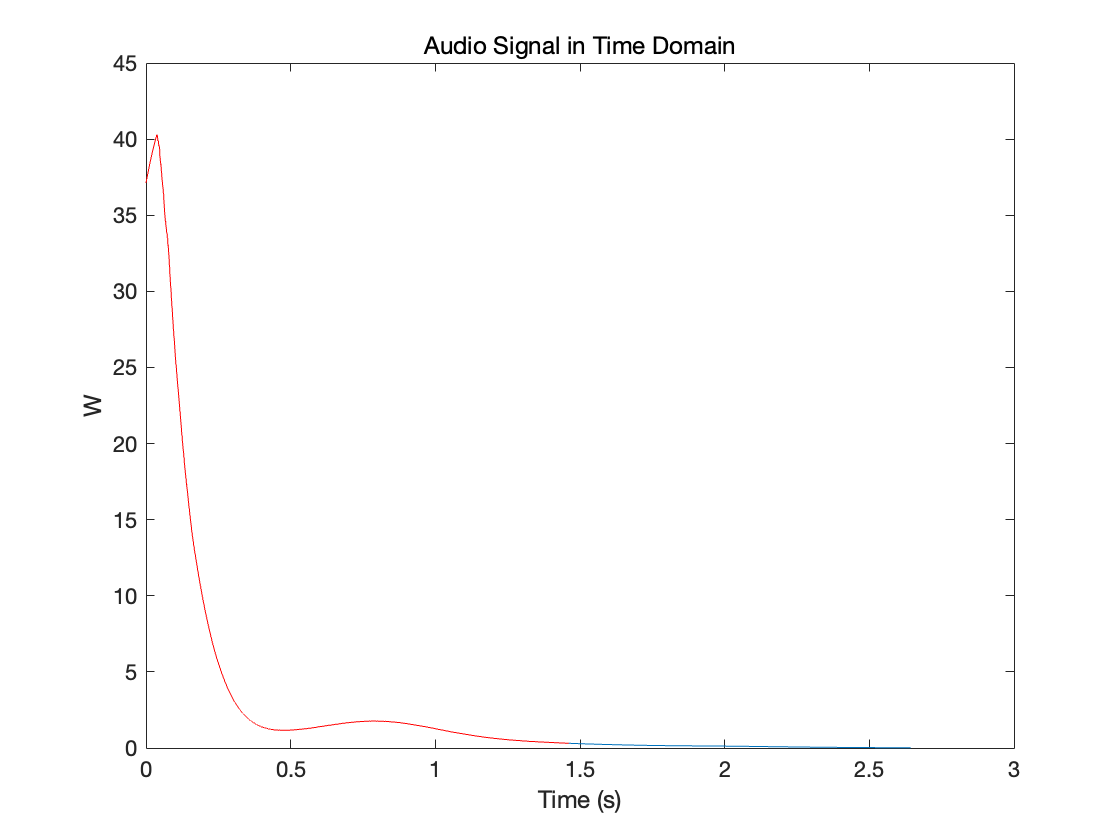
\includegraphics[width=0.8\textwidth]{signal_with_note_detected.png}
    \caption{Exemple signal avec les notes détectées}
    \label{fig:Note_Detection}
\end{figure}
\textcolor{blue}{\subsubsection{Calcul de la puissance moyenne}}

La synchronisation du récepteur est cruciale pour détecter les instants de début et de fin de chaque note. La détection se fait en trouvant les points où la puissance du signal dépasse un seuil défini (1\% de la puissance maximale). Les indices correspondants sont ensuite convertis en temps, fournissant ainsi les instants de début et de fin de chaque note. Les notes d'une durée inférieure à une seconde sont éliminées pour garantir la qualité des données. 
\textcolor{blue}{\subsubsection{Détermination de la Fréquence Fondamentale}}
Le décodage des caractéristiques de chaque note s'effectue en calculant la puissance moyenne, la fréquence fondamentale ($f_0$), la fréquence de la plus haute harmonique ($f_h$), et le nombre d'harmoniques dans la bande de fréquences.La détection précise de la fréquence fondamentale ($f_0$) est essentielle dans l'analyse des signaux sonores, notamment pour l'étude des notes musicales. Ces informations sont extraites à partir du signal audio, utilisant diverses fonctions telles que le calcul de la moyenne de puissance, la fréquence fondamentale par auto-corrélation, et le comptage des harmoniques. Les résultats sont affichés pour chaque note, fournissant une caractérisation détaillée des éléments musicaux contenus chaque fichier audio ainsi que la note et l'octave associée à la fréquence. 

L'ensemble de ces étapes contribue à élaborer un algorithme complet de détection et de caractérisation des notes de musique, avec une option facultative pour estimer la direction de la source sonore sur des signaux acquis par deux micros différents. 

Dans notre étude, nous avons appliqué deux méthodes distinctes pour calculer cette fréquence fondamentale, puis nous les avons comparées afin de vérifier leur exactitude.

La première méthode s'appuie sur la détection de la fréquence qui présente la densité de puissance la plus élevée après avoir effectué une transformation de Fourier rapide (FFT). Cette approche est basée sur l'hypothèse que, dans la majorité des cas, la fréquence fondamentale correspond à la fréquence la plus basse ayant la plus grande densité de puissance.
\begin{equation}
    f_0 = \arg\max_f(\frac{2}{N}|FFT(signal)|)
\end{equation}

Quant à la seconde méthode, nous utilisons le principe de l'auto-corrélation dans le domaine temporel. Cette technique permet de détecter les répétitions périodiques au sein du signal, ce qui facilite l'identification de la fréquence fondamentale, même en présence de harmoniques complexes ou de bruit.
\begin{equation}
    f_0 = \frac{f_s}{Lag_{peak}}
\end{equation}
Où: 
\begin{itemize}
    \item $f_0$ est la fréquence fondamentale  
    \item $f_s$ est la fréquence d'échantillonnage 
    \item $Lag_{peak}$ est le temps de retard correspondant au premier pic significatif de la fonction d'auto-corrélation.
\end{itemize}

Ces méthodes contribuent à élaborer un algorithme complet de détection et de caractérisation des notes de musique. En combinant et en comparant les résultats obtenus par ces deux méthodes, nous pouvons augmenter la fiabilité de notre analyse et assurer une détection plus précise de la fréquence fondamentale, ce qui est crucial pour une compréhension approfondie des propriétés acoustiques des notes analysées.

\textcolor{blue}{\subsubsection{Analyse des Harmoniques}}
Dans l'analyse des signaux audio, la détection précise des harmoniques est essentielle pour comprendre les caractéristiques spectrales du signal.

Notre recherche utilise une méthode basée sur la transformée de Fourier rapide (FFT) pour identifier les composantes harmoniques d'un signal. Ce processus consiste à calculer la FFT du signal et à en extraire les points de fréquence qui répondent à des conditions spécifiques et qui représentent les composantes harmoniques.

Tout d'abord, nous effectuons une FFT sur le signal original pour obtenir son spectre, et nous ne considérons que la partie positive de la fréquence. Dans le spectre, nous identifions d'abord le point de fréquence ayant la puissance la plus élevée (\(P_{max}\)), et à partir de là, un seuil relatif est fixé (typiquement 40 dB en dessous du point de puissance maximale). Tous les points de fréquence supérieurs à ce seuil sont initialement reconnus comme des harmoniques possibles.

Ensuite, pour chaque multiple entier de la fréquence fondamentale (\(n \times f_0 \), où n est un nombre naturel), nous recherchons les points du spectre qui sont les plus proches de ces fréquences. Si les fréquences de ces points ne dépassent pas un seuil de fréquence maximale fixé (\(f_{max}\)) avec une puissance d'au moins 10\% de la puissance maximale, ces points de fréquence sont identifiés comme des harmoniques. De cette manière, nous pouvons extraire efficacement les composants harmoniques du signal.
\begin{equation}
    Harmonics = \{f_n | f_n = n \times f_0, n \in \mathbb{N}, f_n \leq f_{max}, P(f_n) \geq 0.1 \times P_{max} \}
\end{equation}
où :
\begin{itemize}
    \item \(f_n\) est la fréquence de la n-ième harmonique
    \item \(f_0\) est la fréquence fondamentale
    \item \(P(f_n)\) est la densité spectrale de puissance à la fréquence \(f_n\)
    \item \(P_{max}\) est la maxime dans le spectral de fréquence 
    \item \(f_{max}\) est le seuil de fréquence le plus élevé pour la détection des harmoniques
\end{itemize}

\textcolor{blue}{\subsubsection{Extraction et classification des caractéristiques des sons d'instruments de musique}}
Dans le domaine de l'analyse audio numérique, l'extraction des caractéristiques sonores des instruments de musique est essentielle pour la recherche d'informations musicales et la classification des instruments. Nous avons étudié trois caractéristiques clés : le centroïde spectral, le taux de croisements par zéro et l'enveloppe ADSR, ainsi que leur application dans l'identification des types d'instruments.

\textbf{Le centroïde spectral} décrit le centre de gravité du spectre sonore, reflétant la « brillance » du son. Sa représentation mathématique est la suivante : 
\begin{equation}
    C = \frac{\sum_{n=0}^{N-1}f(n)\cdot S(n)}{\sum_{n=0}^{N-1}S(n)}
\end{equation}
où :
\begin{itemize}
    \item \(f(n)\) représente la fréquence
    \item \(S(n)\) l'amplitude correspondante à cette fréquence
\end{itemize}

\textbf{Le taux de croisements par zéro} mesure la fréquence à laquelle la forme d'onde du signal traverse l'axe temporel, et est liée à la hauteur et au timbre du son. Sa formule de calcul est la suivante :
\begin{equation}
    ZCR = \frac{1}{T-1}\sum_{t=1}^{T-1}\frac{1}{2}|\text{sgn}(s(t))-\text{sgn}(s(t-1))|
\end{equation}

\textbf{L'enveloppe ADSR }analyse les variations dynamiques temporelles du son, où chaque phase est définie comme suit :
\begin{itemize}
    \item \textbf{Attack Time(A):}
\end{itemize}
\begin{equation}
    A = \min \{t|s(t)\geq0.9 \cdot P_{peak}, t\in [0, \frac{T}{f_s}]\}
\end{equation}
\begin{itemize}
    \item \textbf{Decay Time(D):}
\end{itemize}
\begin{equation}
    D = \min \{t|s(t)\leq S_{level}, t\in [A, \frac{T}{f_s}] - A\}
\end{equation}
\begin{itemize}
    \item \textbf{Sustain Level (S):}
\end{itemize}
\begin{equation}
    S = \alpha \cdot P_{peak}
\end{equation}
Ou:
\begin{description}
    \item \(\alpha\) est un pourcentage de l'amplitude maximale
    \item \(P_{peak}\) est l'amplitude maximale du signal
\end{description}
\begin{itemize}
    \item \textbf{Release Time (R):}
\end{itemize}
\begin{equation}
    R = \min \{t |s(t) \leq \beta \cdot P_{initial}, t \in [t_{end}, \frac{T}{f_s}]  \} - t_{end}
\end{equation}
Où:
\begin{description}
    \item \(\beta\) est le coefficient qui détermine le seuil d'extinction sonore
    \item \(P_{initial}\) est l'amplitude au début de la phase de libération
    \item \(t_{end}\) est le point où la note se termine
    \item \(T\) est la taille totale de l'échantillon
    \item \(f_s\) est le taux d'échantillonnage
\end{description}

À travers ces caractéristiques, nous avons tenté de classer les instruments de musique. Cependant, nous avons constaté que les résultats de classification n'étaient pas idéaux. Les principales raisons en sont le choix arbitraire des seuils de caractéristiques, la possible superposition des caractéristiques entre différents instruments, ainsi que la complexité due à la diversité des échantillons.

Compte tenu de ces défis, nous estimons qu'il serait plus approprié d'utiliser des méthodes d'apprentissage automatique pour la classification des instruments. L'apprentissage machine, en particulier les techniques d'apprentissage profond, peut automatiquement apprendre des caractéristiques complexes pour distinguer les instruments à partir de grandes quantités de données. Ces méthodes réduisent non seulement le besoin de fixer manuellement des seuils, mais elles permettent également, en apprenant les modèles intrinsèques dans les données, d'améliorer la précision et la capacité de généralisation de la classification.
\textcolor{blue}{\subsection{Résultats Expérimentaux}}
ici est resultats

\textcolor{blue}{\subsection{Conclusion}}
En conclusion, nous avons réussi par le code via Matlab à répondre aux attentes du cahier des charges, c'est à dire à caractériser des notes de musiques. Cette caractérisation passe par la détection de la note jouées, de sa fréquence fondamentale et de son harmonique et de sa puissance moyenne en dBm. Le programme détecte aussi les instants de début et de fin ainsi que le nombre d'harmoniques.

Les résultats à l'exécution du programme sont cohérent avec ce que l'on attend (avec le nom des fichiers qui donnent le nom des notes) et aussi de ce l'on entend.
\newpage
\textcolor{blue}{\section{Chapitre III : Problème III}}
\textcolor{blue}{\subsection{Introduction}}
Nous envisageons la réalisation d'un enregistrement numérique en exploitant un microphone doté d'une sensibilité de S = -47 dBV et capable de capturer des niveaux sonores atteignant 130 dB SPL dans une plage de fréquence de 200 Hz à 20 kHz. En supposant l'absence totale de distorsion et de bruit introduit par le microphone, le signal analogique subit une amplification dont le gain, exprimé en décibels, doit être déterminé. La plage dynamique cible après amplification est fixée à [-1V,+1V]. Après cette étape, le signal est numérisé avec des paramètres spécifiques visant à garantir un rapport signal à bruit d'au moins 40 dB pour un signal acoustique de PdB SPL = 60 dB SPL. Nous entreprenons de déterminer le gain G nécessaire à l'amplification du signal analogique, de fournir un schéma fonctionnel détaillé pour la numérisation, de spécifier tous les paramètres requis, et de calculer le débit du signal numérique résultant. Enfin, nous examinerons la capacité de stockage nécessaire pour enregistrer une heure d'audio en stéréo, évaluerons la compatibilité des paramètres avec la qualité et le stockage sur CD, et analyserons leur aptitude à préserver le timbre des instruments d'un orchestre symphonique.
\newline
\\
\textbf{Problème III - Énoncé } \  \\
On souhaite effectuer un enregistrement numérique en utilisant un micro de sensibilité S = -47 dBV, de niveau sonore maximal de 130 dB SPL de bande passante 200 Hz - 20 kHz. On suppose que ce micro n'introduit aucune distorsion sur la bande considérée et aucun bruit. Le signal analogique est ensuite amplifié avec un gain G (en dB). La dynamique après amplification est [-1V,+1V]. Ce signal est ensuite numérisé. On choisit des paramètres de numérisation afin de garantir un rapport signal à bruit d'au moins 40 dB pour un signal acoustique de PdB SPL = 60 dB SPL.
\\
Déterminer le gain G à appliquer au signal analogique et donner le schéma fonctionnel de numérisation de ce signal, déterminer tous les paramètres et calculer le débit du signal numérique. 
\\
Quelle capacité de stockage faut-il pour enregistrer une heure d'audio en stéréo ? Les paramètres choisis sont-ils compatibles avec une qualité et un stockage sur CD ? Permettent-ils de respecter le timbre des instruments d'un orchestre symphonique ?
\\
Réfléchir sur l'utilité d'adopter un pas de quantification non pas uniforme, mais qui suit une loi logarithmique.
\textcolor{blue}{\subsection{Méthode}}
\textcolor{blue}{\subsubsection{Calcul du gain G à appliquer au signal analogique }}
\input{lectures/Méthodes/Méthode_ProblemIII/Calcul_du_gain_G_à_appliquer_au_signal_analogique }
\textcolor{blue}{\subsubsection{Schéma fonctionnel de numérisation }}
\begin{figure}[htb]
    \centering
    \includegraphics[width=0.8\textwidth]
    % ajouter l'image dans le ficher /pics
    {}
    \caption{Schéma fonctionnel}
    \label{fig:Schéma_Fonctionnel}
\end{figure}
\textcolor{blue}{\subsubsection{Calcul du nombre de bits }}

Pour ce faire, nous utiliserons la formule du rapport signal bruit SNR qui est définie comme :
\begin{equation}
SNR = 10 \log \left( \frac{P_s}{P_b} \right).
\end{equation}
Avec un SNR d'au moins \( 40 \, \text{dB} \), nous déterminons d'abord la puissance du signal utile \( P_s \) puis la puissance du bruit \( P_b \), ce qui nous permet de calculer le nombre de bits.

Reprenons la formule du gain pour déterminer la puissance en dBm :
\begin{equation}
G = P_{\text{dBm}} - S - P_{\text{SPL}} - \left( 30 + 20 \log \left( 20 \times 10^{-6} \right) \right).
\end{equation}
Ce qui nous donne alors :
\begin{equation}
P_{\text{dBm}} = G + S + P_{\text{SPL}} + 30 + 20 \log(P_{\text{ref}}).
\end{equation}

Avec \( P_{\text{SPL}} = 60 \, \text{dB SPL} \) et les mêmes valeurs que pour la partie 3.2.1, nous avons :
\begin{equation}
P_{\text{dBm}} = 11 - 47 + 60 + 30 + 20 \log(20 \times 10^{-6}) \quad \text{donc} \quad P_{\text{dBm}} = -40 \, \text{dBm}.
\end{equation}
\\

Pour convertir la puissance dBm en Watt, appliquons la formule :
\begin{equation}
P_W = 10\log{\left( \frac{P_{\text{dBm}}}{10^{-3}}  \right)} \quad \text{qui peut également être exprimée comme $P_{dBm} = 10\log(1000P_w)$ }.
\end{equation}
En isolant $P_w$, nous obtenons :
\begin{equation}
P_W = 10^{\left( \frac{P_{\text{dBm}}}{10^{-3}}  \right)} \quad \text{ce qui nous donne} \quad P_W = 10^{-7} \, \text{Watt}.
\end{equation}

De plus, nous avons :
\begin{equation}
SNR = 10 \log \left( \frac{P_S}{P_b} \right),
\end{equation}
donc
\begin{equation}
P_b = \frac{P_S}{10^{\frac{SNR}{10}}}.
\end{equation}
La puissance moyenne du bruit de quantification \( P_b \) est donc :
\begin{equation}
P_b = \frac{q^2}{12},
\end{equation}
soit,
\begin{equation}
q^2 = \frac{12 \times P_S}{10^{\frac{SNR}{10}}}.
\end{equation}
De plus, \( q \) est donné par :
\begin{equation}
q = \frac{2A}{2^b},
\end{equation}
donc
\begin{equation}
\left( \frac{2A}{2^b} \right)^2 = \frac{12 \times P_S}{10^{\frac{SNR}{10}}},
\end{equation}
et
\begin{equation}
A^2 \times 2^{2(1-b)} = \frac{12 \times P_S}{10^{\frac{SNR}{10}}}.
\end{equation}
Ainsi, nous avons :
\begin{equation}
2^{2(1-b)} = \frac{12 \times P_S}{A^2 \times 10^{\frac{SNR}{10}}},
\end{equation}
et en terminant les calculs :
\begin{equation}
2(1-b) = \log_2 \left( \frac{12 \times P_S}{A^2 \times 10^{\frac{SNR}{10}}} \right),
\end{equation}
puis
\tcbox[colback=green!20, colframe=green, boxrule=2pt]{$b = 1 - \frac{\log_2 \left( \frac{12 \times P_S}{A^2 \times 10^{\frac{SNR}{10}}} \right)}{2}$}
Avec A = 1V, SNR = 40 dB, et $P_s = 10 ^{-7} W$, nous obtenons b $\approx 17.47.$
\\
Nous savons que les bits prennent des valeurs entières, ainsi, nous avons donc \tcbox[colback=green!20, colframe=green, boxrule=2pt]{18 bits.}


\
\textcolor{blue}{\subsubsection{Calcul de la capacité de stockage pour enregistrer une heure d’audio en stéréo}}
Nous avons $D = F_e * b$
\\
Où D est le débit binaire, $F_e$ la fréquence d'échantillonnage, b le nombre de bits.
\\
En considérant nos paramètres, avec une bande passante 200 Hz à 20 kHz, la fréquence d'échantillonnage $F_e$ doit être d'au moins 40 000 Hz, conformément au théorème d'échantillonnage de Shannon, où nous devons respecter $F_e\ge 2F_{max}$ avec $F_{max}$ étant égal à 20 kHz. Ainsi $F_e$ doit être d'au moins 40 kHz. Pour le nombre de bits b, nous avons 18 bits, enfin, il faut multiplier le débit par 2, car nous sommes en stéréo. 
\\
Ainsi, après calculs, nous avons
\tcbox[colback=green!20, colframe=green, boxrule=2pt]{$C_s = \frac{3600*40 000*18*2}{8} = 648 M_o$}

Cependant, nous ne sommes pas certains d'être en stéréo, alors nous effectuons le même calcul en considérant le cas où nous sommes en mono.
\\
Après les calculs, nous obtenons \sethlcolor{green}\hl{$C_m = \frac{3600*40 000*18}{8} = 324 M_o$}
\textcolor{blue}{\subsubsection{Compatibilité avec une qualité et un stockage sur CD}}
La fréquence d'échantillonnage $F_e$ pour un CD standard est déjà établie à 44 100 Hz, tout comme le nombre de bits b qui est 16 bits et l'enregistrement sur CD se fait en stéréo.(1)
\\
Ainsi, \\
\tcbox[colback=yellow!20, colframe=yellow, boxrule=2pt]{$D = 44.1*10^3*16*2 = 1 411 200 
 bit/s$}
\\
La capacité $C_{CD}$ est exprimée par $C_CD = D * d$, où D représente le nombre binaire et d la durée que nous avons sélectionnée, correspondant à 1 heure, soit 3 600 secondes.
\\
En effectuant une division par 8 pour obtenir le résultat en octet, la capacité $C_CD$ se calcule comme suit : \tcbox[colback=green!20, colframe=green, boxrule=2pt]{$C_CD = \frac{1 411 200*3600}{8} \approx 635 M_o$}
\\
Ainsi, la capacité de stockage nécessaire pour enregistrer une heure d'audio en stéréo sur un CD standard est d'environ 635 $M_o$.
\\

Par conséquent, avec nos paramètres choisis, l'enregistrement \uline{n'est pas conforme aux spécifications d'un CD audio standard}, \textbf{si on est dans le cas où nous sommes en stéréo}. Il pourrait être envisageable d'explorer d'autres supports ou formats offrant une flexibilité plus grande pour répondre à des exigences spécifiques en termes de bande passante et de qualité audio. Sinon, dans le cas où \textbf{nous sommes en mono}, \uline{cela est conforme aux spécifications d'un CD audio standard}.
\\
\scriptsize{source :}
1. Cours de cycle préparatoire associé avec Stanislas
\normalsize

\textcolor{blue}{\subsubsection{Respect de la fidélité du timbre des instruments d'un orchestre symphonique}}
Pour récupérer de la musique avec fidélité, il convient de conserver le timbre musical, autrement dit, garder le plus d'harmoniques possibles, et pas uniquement le fondamental. Autrement dit, plus la fréquence d'échantillonnage est élevée, et plus nous avons de chance de respecter le timbre \footnote{\href{https://fr.wikipedia.org/wiki/Gain_d\%C3\%A9cibel}{Cliquez ici pour accéder à la source sur le timbre}} d'un instrument. 
\\Prenons un orchestre symphonique possédant une harpe, la plus haute note jouée avec cet instrument est un sol dièse 7 (3322.4 Hz)\footnote{\href{http://hyperphysics.phy-astr.gsu.edu/hbase/Music/orchins.html}{Cliquez ici pour accéder à la source de la fréquence de sol dièse 7 d'une harpe}}. Notre bande passante est de 20 000 Hz, nous pouvons donc récupérer 5 harmoniques d'un sol dièse 7 plus la fondamentale (nous atteignons alors 19 934.4 Hz).
\\De plus, comme précisé dans la partie 3.2.4, notre fréquence d'échantillonnage doit être au moins deux fois plus grande pour éviter le repliement spectral, ainsi, nous pouvons estimer que nous respecterons le timbre des instruments de musique dans un orchestre symphonique, et récupérer suffisamment d'harmonique de cet orchestre. L'oreille humaine ne pouvant pas réellement distinguer les sons au-delà de 14 000 Hz, cela est suffisant.
\\De surcroît, nous avons calculé un nombre de bits de quantification égale à 18. Ce nombre de bits est suffisamment élevé pour réduire au plus possible le bruit de quantification. En vérité, si le CD reste peu aimé pour l'écoute de musique classique\footnote{\href{https://www.radiofrance.fr/franceculture/podcasts/hashtag/la-musique-classique-peut-elle-encore-resister-a-la-dematerialisation-7501004}{Cliquez ici pour accéder à la source sur la musique la classique}}, c'est plus par appréciation de l'unité des performances d'un orchestre, ou par le fait de ne pas aimer le support  lui-même, mais la qualité d'enregistrement ne semble pas un problème. Le CD standard a 16 bits de quantification, nous pouvons conclure que le timbre des instruments d'un orchestre sera respecté.


\textcolor{blue}{\subsubsection{Réflexion sur l’utilité d’un pas de quantification qui suit une loi logarithmique}}
En règle générale, on adopte un pas de quantification uniforme pour échantillonner de l'information qui suit elle-même une distribution uniforme. Cependant, les signaux sonores ne suivent pas de distribution uniforme. Cependant, les signaux sonores ne suivent pas de distribution uniforme, il peut être utile d'adopter un pas de quantification suivant une loi logarithmique pour minimiser les distorsions (bruit de quantification). Il existe d'ailleurs un algorithme permettant de déterminer le pas de quantification idéal, l'algorithme de Lloyd-Max.
\\
\scriptsize{source :}
\href{https://fr.wikipedia.org/wiki/Quantification_%28signal%29}{Ce lien}

\normalsize
\textcolor{blue}{\subsection{Conclusion}}
En conclusion, notre démarche vise à réaliser un enregistrement numérique à partir d'un microphone. Après avoir déterminé un gain optimal de 11 dB et un nombre de bits de 18, nous avons calculé une capacité de stockage estimée de 648 $M_o$ pour 1 heure d'audio en stéréo.
\\

Cependant, l'estimation de la capacité de stockage, à 648 $M_o$ pour une heure d'audio en stéréo, présente une légère divergence par rapport à la norme d'un CD standard, fixée à 635 $M_o$. Cette différence souligne la complexité de l'équilibre entre la qualité audio et la contrainte de stockage, ce qui pourrait rendre une telle configuration incompatible avec un CD standard.
\\

Il est important de noter toutefois que si l'enregistrement est effectué en mono, notre approche pourrait être compatible avec les spécifications d'un CD standard. Cela met en lumière l'importance de considérer la configuration audio choisie lors de l'évaluation de la compatibilité avec les normes de stockage existantes. De plus, la réflexion sur l'adoption d'un pas de quantification logarithmique a ouvert des perspectives innovantes pour optimiser la représentation des signaux, en particulier à faible amplitude, tout en minimisant les distorsions.
\\

Notre approche méthodologique, du choix de gain à la réflexion sur la quantification, établit une base solide pour des ajustements futurs visant à concilier au mieux qualité sonore et contraintes de stockages dans des contextes spécifiques.
\newpage
\textcolor{blue}{\section{Chapitre IV : Problème IV}}
\textcolor{blue}{\subsection{Introduction}}
\textbf{Problème IV - Énoncé } \ \\
On souhaite détecter les signaux environnementaux qui comprennent des composantes spectrales très aiguës et pénibles pour l'oreille humaine. Ces signaux sont définis ainsi : 20\% de leur puissance est comprise dans les fréquences supérieures à 2 kHz, avec une puissance sonore totale supérieure à 110 dB SLP. \\
Concevoir un système de détection de ces signaux pénibles fondé sur filtrage
numérique. On prendra un micro de sensibilité égale à -67 dBV et de gain égal à 16 dB. Discuter les critères énoncés.

\textcolor{blue}{\subsection{Méthode}}
\textcolor{blue}{\subsection{Résultats Expérimentaux}}
\textcolor{blue}{\subsection{Conclusion}}

\end{document}